%% ----------------------------------------------------------------
%% Conclusions.tex
%% ---------------------------------------------------------------- 


%\chapter{Conclusions} \label{Chapter: Conclusions}
\section{Conclusions} \label{Section: Conclusions}

During this project a systemverliog program was successfully implemented on FPGA device to perform the affine transform with designated matrix constants. During the process the picoMIPS architecture was well studied, including the understanding of the function of each module, the usage of the synchronous and asynchronous RAM, top level CPU design, instructions design and so on. Meanwhile, experience was gained in using synthesis tool and programmer Quarter II.\\\\
At the second stage of the development, the processor was optimized with usage of synchronous RAM and the cost figure of the system was significantly reduced. The number of logic units used in the original design and improved one are summarized in Figure {fig:cpucost}. 

\begin{figure}[H]
		\centering
		%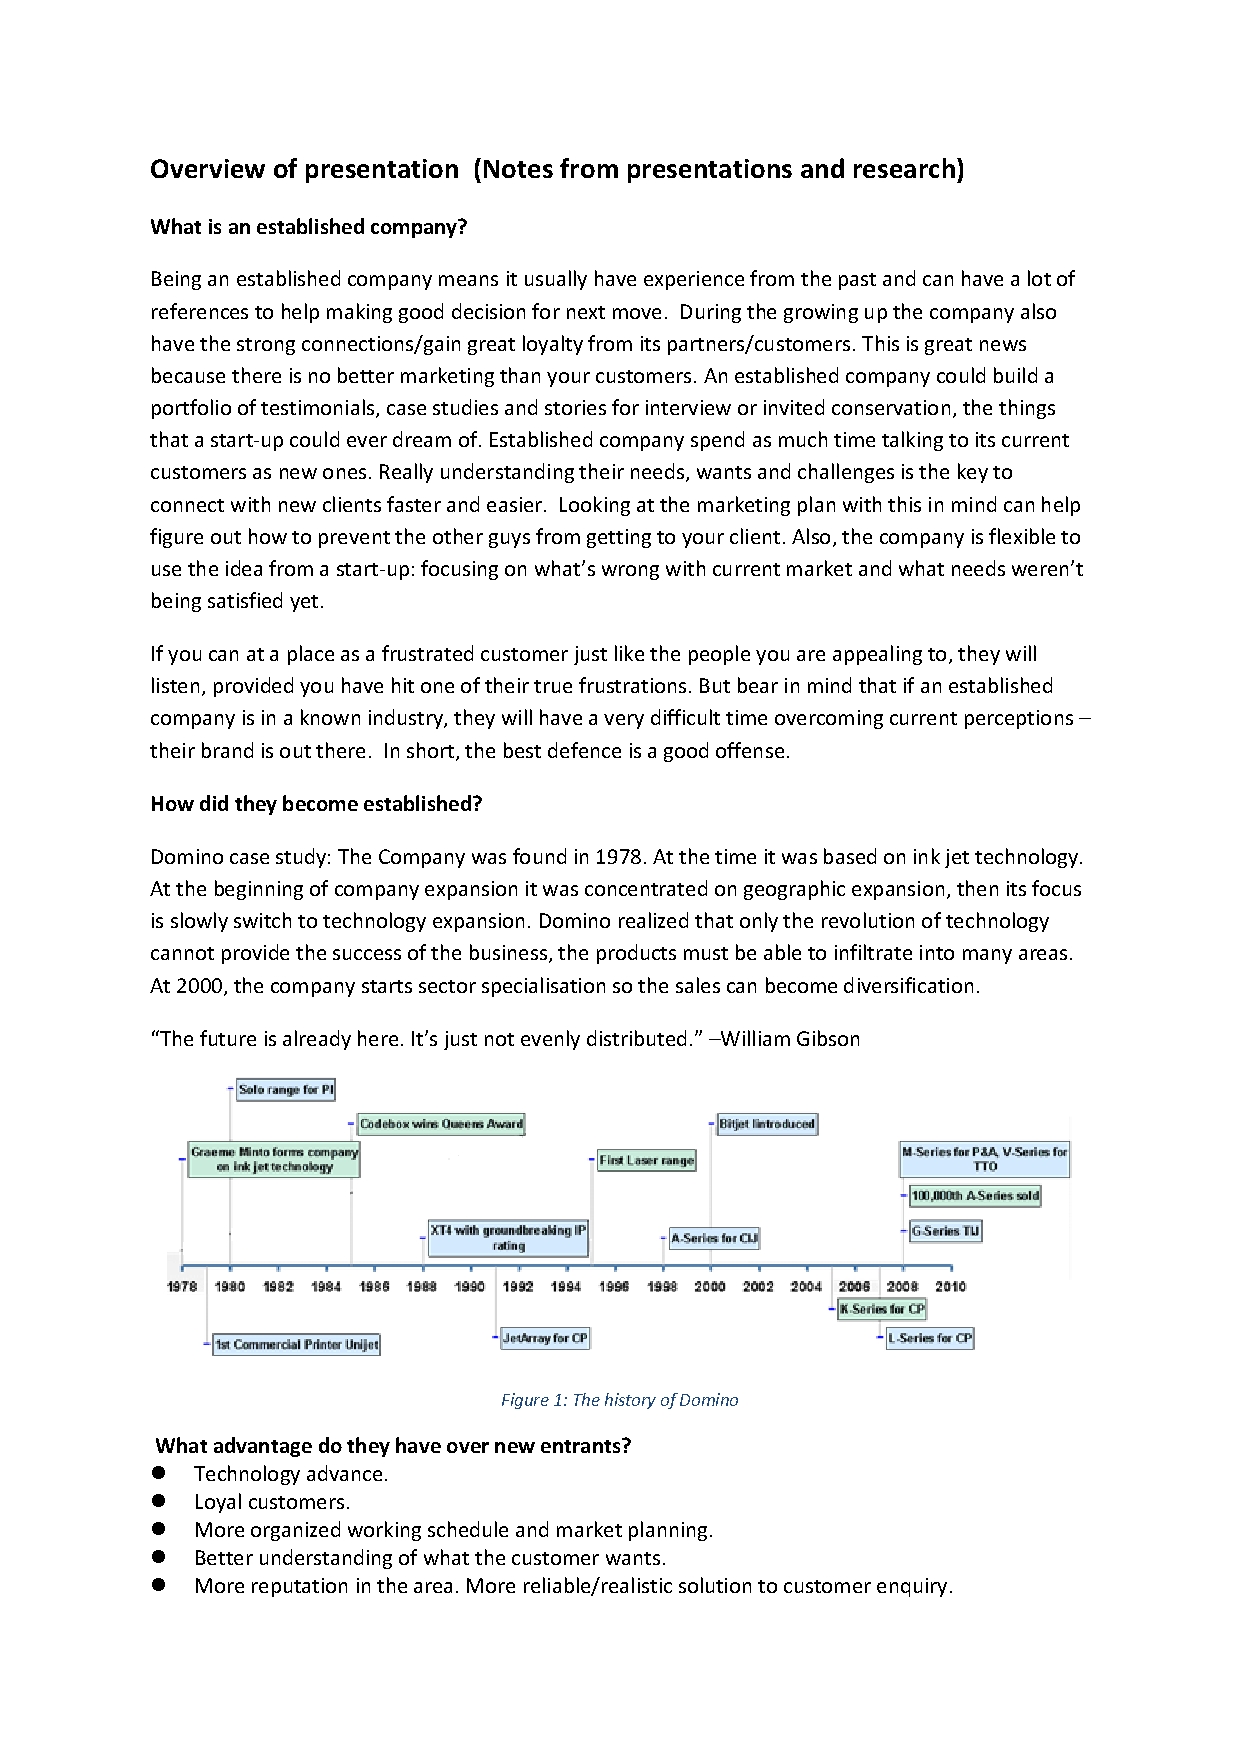
\includegraphics[width = 0.9\textwidth]{Figures/Overview_of_presentations}
		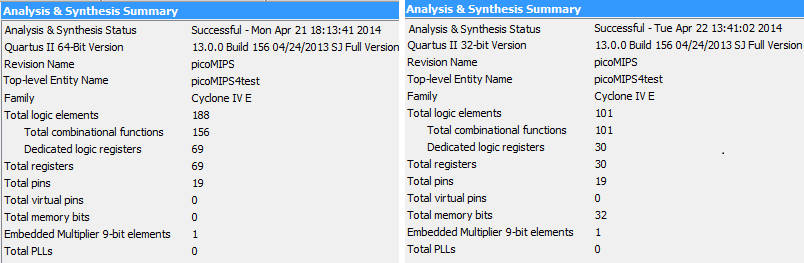
\includegraphics[width = \textwidth]{Figures/cpucost}		
		\caption{Logic elements usage of original and improved CPU, including slow clock counter. (\textit{Left}: Origianl CPU \textit{Right}: Improved CPU)}
		\label {fig:cpucost}
\end{figure}
The cost figure of original design is \(132 + 30 \times 0 = 132 \). \\
The improved one is \(76 + 30 \times 0.03125 \approx 76.94 \).  \\
The percentage of reduction is 42\%.\\\\
The future work could focus on reducing the instructions in the program memory in the case that the affine transform will be combined within other operations, even though this improvement may increase the complexity of other modules. To reduce the size of ALU, the addition operation could be divided out of it to save a 8bits multiplexer. Same operation could be done by an accumulator added after the ALU, at the cost that adding one more clock cycle delay to the already slow system and changing the whole architecture dramatically. An alternative approach would be introducing the pipeline to improve the calculation efficiency.

